%# -*- coding: utf-8-unix -*-
% !TEX program = xelatex
% !TEX root = ../thesis.tex
% !TEX encoding = UTF-8 Unicode

% how to evaluate?
% random picking relation, labeling true or false?
% the count precision@x?

% check: 1. GY's paper
%        2. ritter's paper

% Check their page size
% write about our size.
% and compare the version of MI-Equal, MI-Uniform, TfIdf-Equal, TfIdf-Uniform
%%In the demonstration part, we first introduce the experimental setup.
%%Secondly we evaluate the accuracy of relation type inferring.
%%Then we present our web interface of RvSp system, and finally
%%we provide some example relations with the inferred argument types.

\subsection{实验}
\label{sec:tinf-exp}
% Add Freebase dump citation
%\KZ{First, say a bit about the ReVerb dataset, and the specifics of
%Freebase. Then say something about our implementation details in the
%3 steps, such as parser we used, etc. What about the numbers in the table?}

\subsubsection{实验设置}
我们在实验中使用的知识库为Freebase\cite{bollacker2008freebase}在2014年2月16日的版本,
包含了大约40,000,000个不同实体,以及1,700个主要类型。
%\footnote{Freebase的每个类型都对应一个id,例如``professional athlete''
%在知识库中的类型id为$sports.pro\_athlete$。}。
实验中使用的开放式信息抽取系统为ReVerb\cite{fader2011identifying},
ReVerb数据集提供了多种版本,我们使用的版本包含了置信度最高的14,000,000个关系三元组。
%Each entity belongs to at least one type.
%When compared with other knowledge bases, Freebase has a much greater focus on named entities than {\tt WordNet}.
%Besides, the type hierarchy of {\tt Yago} is too fine-grained, which is not suitable for schema inferring.
%Considering aspects mentioned above, we adapt Freebase as our knowledge base in our work.
%The input ReVerb dataset is released by Lin et al.\shortcite{lin2012entity}, containing 3 millions of relation tuples with high quality.

ReVerb抽取的三元组中,部分关系参数无法链接到Freebase中的某一个实体,
例如三元组($Metro\ Manila,\ consists\ of,\ \textbf{12 cities}$),
其宾语显然不是一个实体,而是用自然语言描述的类型。
这部分三元组不是我们的研究对象,需要进行过滤。
考虑到在自然语言中,概念通常对应非专有单词,并且多为小写,
因此我们根据WordNet收集了常用的非专有单词。
若一个三元组中包含纯小写,或纯粹由非专有单词构成的主宾语,
那么该三元组将被过滤。
除此之外,ReVerb三元组中还具有时间或日期作为关系参数的情况,
例如 ``Jan. 16th, 1981'' 作为宾语,但同样不对应Freebase的某个实体。
为应对这种情况,我们使用SUTime\cite{chang2012sutime}工具识别
时间或日期,将它们替换为具有$type.datetime$类型的虚拟实体。
经过清理之后,系统共收集了3,234,208个三元组,
对应171,168个不同的关系分组。

% Talk about entity linking.
%We make the following parameter settings by empirics:
%The following parameters are tuned using a development set:
实验中具体使用的参数值为:
$\tau = 0.667$,$\rho = e^{-50}$,
$\epsilon=0.6$以及$\lambda = 5\%$。
关系分组步骤中,我们使用Stanford Parser\cite{klein2003accurate}
对每个关系进行词性标注、语法分析以及时态转换。
%All the data sets involved in the evaluation are available at
%\url{http://202.120.38.146/schema/}.



\subsubsection{结果分析}
我们首先对实体链接进行评测。
由于ReVerb没有提供主宾语的链接结果,
我们从所有关系实例中随机挑选200个三元组,并人工标注这些主宾语所链接的实体。
我们对比实体链接过程的朴素方法和集成方法,
使用准确率(Precision),召回率(Recall),$F_1$分值,以及MRR\cite{liu2009learning}
作为评价指标。
MRR为平均排名倒数(Mean Reciprocal Rank),
即统计正确的链接结果在输出列表中的排名,再计算所有三元组上排名倒数值的平均。
当一个三元组的主宾语均链接正确时,我们才认为该三元组链接正确。
实验结果比较如\tabref{tab:tinf-linking}所示。
不同于常规文本的实体链接,由于每个三元组的上下文极少,链接具有一定难度。
基于集成的链接方法引入了关系与实体间语义的匹配模型,
使主宾语的链接实体互相影响,
链接过程的准确率和召回率均得到稳定提升。

%We assigned 3 human annotators to judge whether both arguments are linked to correct entities.
%We don't have a gold set for entity linking, but we assume that each unlinked relation tuple corresponds to a linked tuple.
%Therefore, we can approximate the recall of entity linking as:
%\begin{equation}
%recall\ =\ \frac {precision * \#Linked\ Tuples} {\#Relation\ Tuples}
%\end{equation}
%For each strategy, the total number of linked tuples, precision, recall and F1 are listed in \tabref{tab:linking_result}.

\begin{table}[ht]
	\centering
	\bicaption{ReVerb三元组的实体链接实验结果。}{Entity linking result.}
	\begin{tabular}{c|cccc}
		%\toprule
        \hline
	    Linking Strategy & Precision & Recall & $F_1$ & MRR \\
        \hline
        Naive    & 0.371 & 0.327 & 0.348 & 0.377 \\
        Ensemble & 0.386 & 0.340 & 0.361 & 0.381 \\
        \hline
	\end{tabular}%
	\label{tab:tinf-linking}%
\end{table}


接下来我们衡量二元关系的主宾语搭配结果,主要关注具有较多实例的关系分组。
我们首先从包含至少500个三元组的关系分组中,随机选择50个分组,
对于每个分组,我们挑选出支持集合数量最大的100个类型对作为评测的对象。
我们将这些类型对分配给3位对Freebase类型有了解的标注者,
每个标注者根据自己的理解,判断类型对是否适合于描述对应关系,
并标注0到3的分值。
将三位标注者的打分进行平均,即可得到这50个关系分组的类型对排序。

我们使用点对点互信息(Pointwise Mutual Information)\cite{church1990word}
作为基线模型,该模型在选择偏好任务中被使用,例如文献\parencite{resnik1996selectional}。
PMI模型使用以下公式定义一个关系$r$与类型对$tp$的关联度:
\begin{equation}
PMI(r, tp) = p(r, tp) \log \frac {p(r, tp)}{p(r, *) p(*, tp)},
\end{equation}
其中$p(r, tp)$代表联合概率,即关系分组为$r$,且支持$tp$的三元组占所有三元组的比重,
$*$代表任意关系或类型对。

我们使用MRR分数进行评测,衡量不同方法生成的最佳关系模式在标注列表中的位置。
如\tabref{tab:tinf-mrr}所示,和基线模型进行比较,
我们的方法在MRR指标上获得了10.1\%的相对提升。

\begin{table}[ht]
	\centering
	\bicaption{二元关系模式推理的评测结果。}{End-to-end schema inference results.}
	\begin{tabular}{c|c}
        \hline
		Approach & MRR Score \\
        \hline
        PMI Baseline & 0.306 \\
        Our Approach & 0.337 \\
        \hline
	\end{tabular}%
	\label{tab:tinf-mrr}%
\end{table}

%\begin{figure%}[htp]
%\centering \scalebox{0.6}{\includegraphics{eval.eps}}
%%\epsfig{file=figure1-cropped.eps, width=2\columnwidth}
%%\scalebox{0.35}
%\caption{Average precision at different ranks.}
%\label{fig:precision}
%\end{figure}

% We randomly sample K relations, use 3 annotators to annotate whether a type pair is true or not.
% count precision@px

%\subsection{Web Interface}
%In addition, we set up a website \footnote{http://202.120.38.146/rvsp} for users to query the schemas of a binary relation.
%Users can search for type pairs by providing the binary relation alone, or the relation with the type of either arg1 or arg2.
%The interface will output the ranked list of schemas satisfying the input constraint along with its support instances.
%Before querying, the interface will transform the relation pattern, using the method introduced in section 4.

%Due to argument types in RvSp is recognized by Feebase type id, which doesn't match its name exactly, we provide typing suggestion in the web interface, %making users easily enter Freebase types.
%Users can browse Freebase website \footnote{http://www.freebase.com} for detail information about type id.

%
%\\
%\\
%
%\begin{figure}[ht]
%\centering
%\epsfig{file=cropped-demo1.eps, width=0.6\columnwidth, angle=270}
%\caption{Query Interface}
%\label{fig:demo1}
%\end{figure}
%
%
%\figref{fig:demo1} shows the result page.
%User can click ``page up'' and ``page down'' to check more results.
%Besides, for each relation schema, user can click ``detail'' link too check all its support tuples.
%The schema details are shown in \figref{fig:demo2}.
%\\
%\\
%
%\begin{figure}[ht]
%\centering
%\epsfig{file=cropped-demo2.eps, width=0.6\columnwidth, angle=270}
%\caption{Schema Details}
%\label{fig:demo2}
%\end{figure}
%

最后,\tabref{tab:tinf-sample}列举了一些具体的关系分组,
以及我们系统抽取的关系模式。
我们可以看出,当构建了Freebase的类型层次结构之后,
系统能够同时得到粗粒度和细粒度的类型信息,
因此最终生成的类型对具有更加丰富的信息量。


%
%\begin{table*}[htbp]
%	\centering
%	\caption{Sample Relation Schemas}
%	\begin{tabular}{Ic|l|lI}
%		%\toprule
%        \whline
%		Relation & Arg1 Type & Arg2 Type \\
%        \whline
%        & book.author & book.book \\
%        & book.author & book.written\_work \\
%        be the writer of & tv.tv\_writer & award.award\_nominated\_work \\
%        & people.person & book.book \\
%        & people.person & book.written\_work  \\
%        \hline
%        & fictional\_universe.fictional\_character & tv.tv\_actor  \\
%        & fictional\_universe.fictional\_character & film.actor  \\
%        be play by & fictional\_universe.fictional\_character & people.person  \\
%        & fictional\_universe.fictional\_character & influence.influence\_node  \\
%        & people.person & tv.tv\_actor  \\
%        \hline
%        & organization.organization\_founder & organization, organization \\
%        & people.person & organization, organization \\
%        found & people.deceased\_person & organization, organization \\
%        & organization.organization\_founder & business.business\_operation \\
%        & organization.organization\_founder & business.employer \\
%        \whline
%	\end{tabular}%
%	\label{tab:sample_relation}%
%\end{table*}
\begin{table}[ht]
	\centering
	\bicaption{生成的二元关系模式举例。}{Real examples of generated relation schemas.}
	\begin{tabular}{c|c}
        \hline
		Relation & Top-3 schemas \\
        \hline
        & $\langle location,\ location \rangle$ \\
        be found at & $\langle employer,\ location \rangle$ \\
        & $\langle organization,\ location \rangle$\\
        \hline
        & $\langle person,\ tv\ program \rangle$\\
        appear on & $\langle person,\ nominated\_work \rangle$\\
        & $\langle person,\ winning\ work \rangle$\\
        \hline
        & $\langle person,\ nominated\_work \rangle$\\
        be the writer of & $\langle person,\ film \rangle$\\
        & $\langle person,\ book\_subject \rangle$\\
        \hline
	\end{tabular}%
	\label{tab:tinf-sample}%
\end{table}

